\documentclass{article}


\PassOptionsToPackage{square,comma,numbers,sort&compress}{natbib}

% Keep this line uncomment in the first submission
\usepackage{neurips_2024} 

%Uncomment this line for the second submission
%\usepackage[final]{neurips_2024}

\usepackage{graphicx}
\usepackage{caption}
\usepackage{subcaption}
\usepackage[utf8]{inputenc} % allow utf-8 input
\usepackage[T1]{fontenc}    % use 8-bit T1 fonts
\usepackage[hidelinks]{hyperref}       % hyperlinks
\usepackage{url}            % simple URL typesetting
\usepackage{booktabs}       % professional-quality tables
\usepackage{amsmath}
\usepackage{amssymb}
\usepackage{amsfonts}       % blackboard math symbols
\usepackage{nicefrac}       % compact symbols for 1/2, etc.
\usepackage{microtype}      % microtypography
\usepackage{xcolor}         % colors
\usepackage{physics}
\usepackage{enumerate}


% koden
\definecolor{codegreen}{rgb}{0,0.6,0}
\definecolor{codegray}{rgb}{0.5,0.5,0.5}
\definecolor{codepurple}{rgb}{0.58,0,0.82}
\definecolor{backcolour}{rgb}{0.95,0.95,0.92}
\usepackage{listings}
\lstdefinestyle{mystyle}{
backgroundcolor=\color{backcolour},
commentstyle=\color{codegreen},
keywordstyle=\color{magenta},
numberstyle=\tiny\color{codegray},
stringstyle=\color{codepurple},
basicstyle=\footnotesize\ttfamily,
breakatwhitespace=false,
breaklines=true, captionpos=b,
keepspaces=true, numbers=left,
numbersep=5pt, showspaces=false,
showstringspaces=false,
showtabs=false, tabsize=2,
}
\lstset{style=mystyle}

\definecolor{codegreen}{rgb}{0,0.6,0}
\definecolor{codegray}{rgb}{0.5,0.5,0.5}
\definecolor{codepurple}{rgb}{0.58,0,0.82}
\definecolor{backcolour}{rgb}{0.95,0.95,0.92}
\usepackage{listings}
\lstdefinestyle{mystyle}{
backgroundcolor=\color{backcolour},
commentstyle=\color{codegreen},
keywordstyle=\color{magenta},
numberstyle=\tiny\color{codegray},
stringstyle=\color{codepurple},
basicstyle=\footnotesize\ttfamily,
breakatwhitespace=false,
breaklines=true, captionpos=b,
keepspaces=true, numbers=left,
numbersep=5pt, showspaces=false,
showstringspaces=false,
showtabs=false, tabsize=2,
}
\lstset{style=mystyle}

\bibliographystyle{abbrvnat}

\title{Do we need more bikes?\\
Project in Statistical Machine Learning}

\author{
  Erik ~Björk\\
  \AND
  Simona ~Stoyanoska
  \AND
  Olov ~Rahm\\
  \AND
  Jakob ~Hanson\\
}
\makeatletter
\renewcommand{\@noticestring}{}
\makeatother
\graphicspath{{./bilder/}}





% -------------------- HÄR BÖRJAR DOKUMENTET -------------------
\begin{document}


\maketitle

\begin{abstract}
  In this project we develop, and study different statistical machine learning models for predicting whether the number of available bikes at a given hour should be increased, a project by the District Department of Transportation in Washington D.C. The training data set consists of 1600 instances of hourly bike rentals, and a test set of 400 instances. The models for prediction we have used are: \emph{Logistic regression, Discriminant methods: LDA, QDA, $k$- Nearest Neighbour}, and \emph{Tree Based Methods}. We have found that T$k$- Nearest Neighbour gives best prediction, with accuracy 92 \%.
\end{abstract}

%\documentclass{article}
\usepackage{graphicx} % Required for inserting images

\title{Planing for project}
\author{Olov Rahm}
\date{January 2025}

\begin{document}

\maketitle

\noindent
(i) Explotre and preprocess data
\\
(ii) try some or all classification methods, which are these?
\begin{itemize}
    \item Support-vector machine?
\end{itemize}
(iii) Which of these are to be "put in producion"?

\end{document}

%%%%%%%%%%%%%%%%%%%%%%%%%%%%%%%%%%%%%%
%%%%%%%%%%%%%%%%%%%%%%%%%%%%%%%%%%%%%%
%%%%%%%%%%%%%%%%%%%%%%%%%%%%%%%%%%%%%%
%%%%%%%%%%%%%%%%%%%%%%%%%%%%%%%%%%%%%%
%%%%%%%%%%%%%%%%%%%%%%%%%%%%%%%%%%%%%%
\section{Introduction}
Statistical machine learning is a subject that aims to build and train algorithms, that analyse large amount of data, and make predictions for the future, which are computed by using established statistical models, and tools from functional analysis. This is a project in supervised, statistical machine learning, where several models were created, and trained, in order to analyse which one of them gives best prediction for the project "Do we need more bikes", where we want to understand, and predict if there is a high, or low demand of city bikes in the public transportation of Washington, a project by the District Department of Transportation in Washington D.C..

The data set used for training our models, consist of 15 variables, containing quantitative/qualitative data. We developed several models, and evaluated them with cross-validation, in order to understand which algorithm gives the best prediction. 
\section{Data Analysis}
In the data, there are some numerical and categorical features:
\begin{itemize}
    \item \emph{Numerical}: \texttt{temp}, \texttt{dew}, \texttt{humidity}, \texttt{precip}, \texttt{snow}, \texttt{snowdepth}, \texttt{windspeed}, \texttt{cloudcover} and \texttt{visibility}.
    \item \emph{Categorical}: \texttt{hour\_of\_day}, \texttt{day\_of\_week}, \texttt{month}, \texttt{holiday}, \texttt{weekday}, \texttt{summertime}, and \texttt{increase\_stock}
\end{itemize}

\begin{figure}[htbp]
    \centering
    \begin{subfigure}{0.45\textwidth}
        \centering
        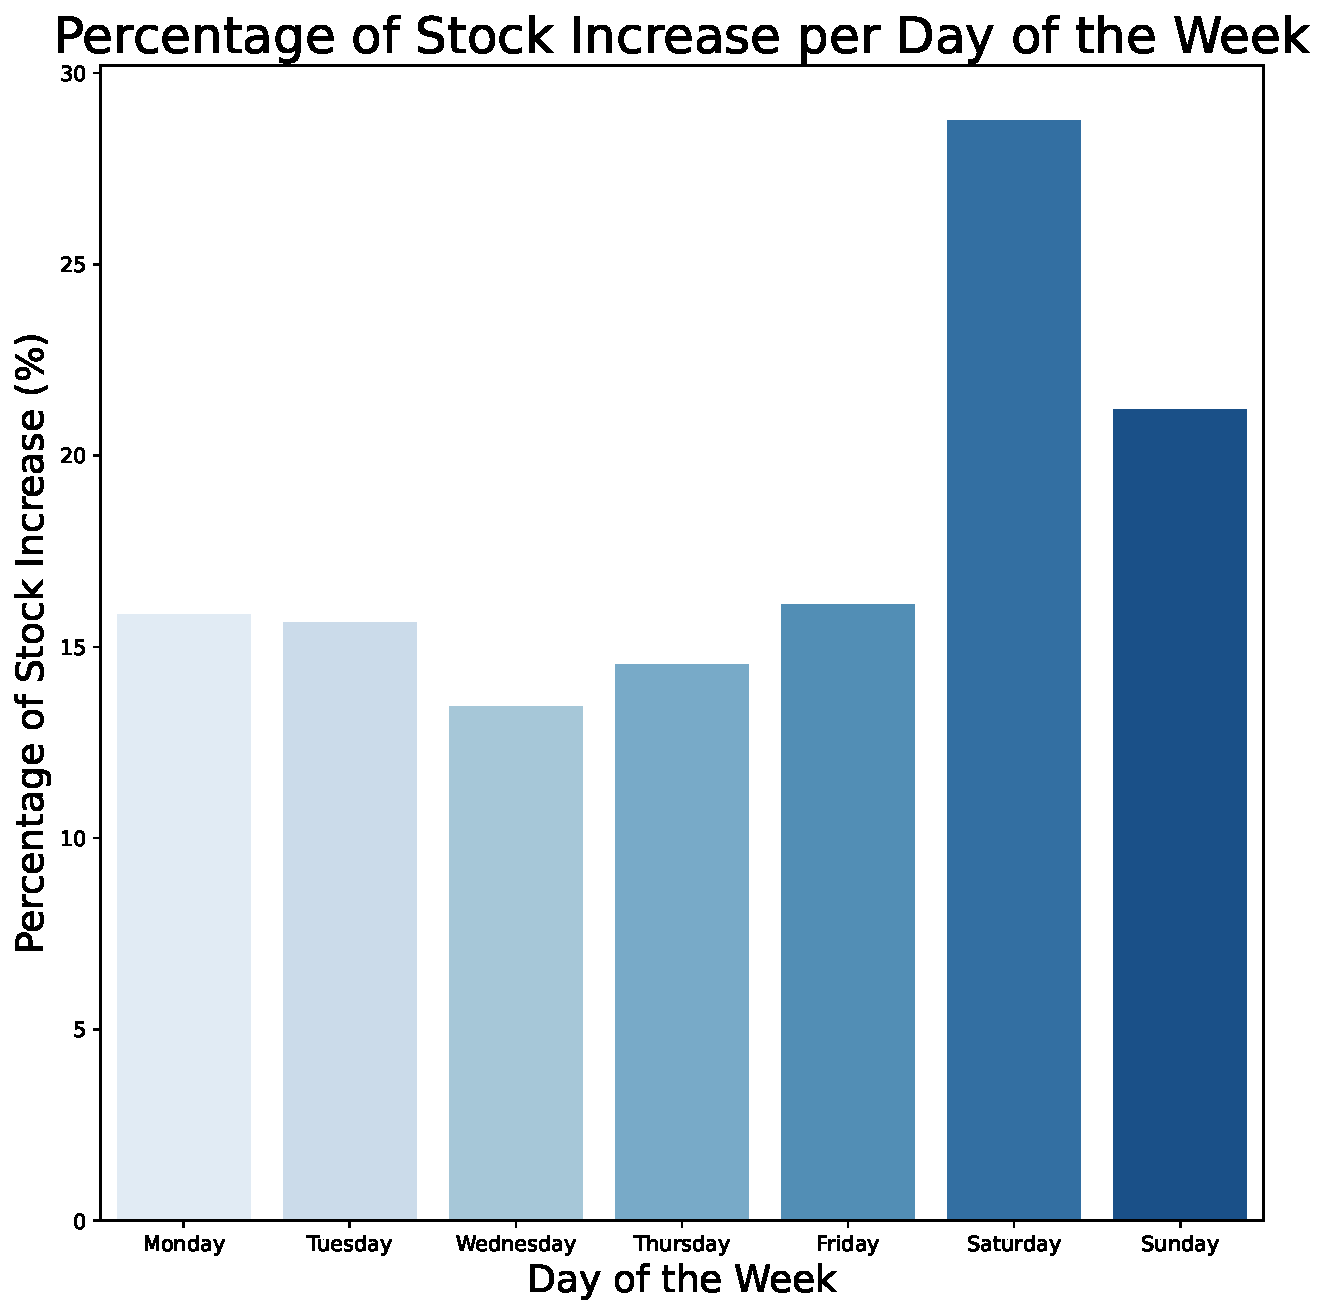
\includegraphics[width=\textwidth]{demand_day.pdf}
        \caption{Demand per day of week.}
        \label{fig:demand day}
    \end{subfigure}
    \hfill
    \begin{subfigure}{0.45\textwidth}
        \centering
        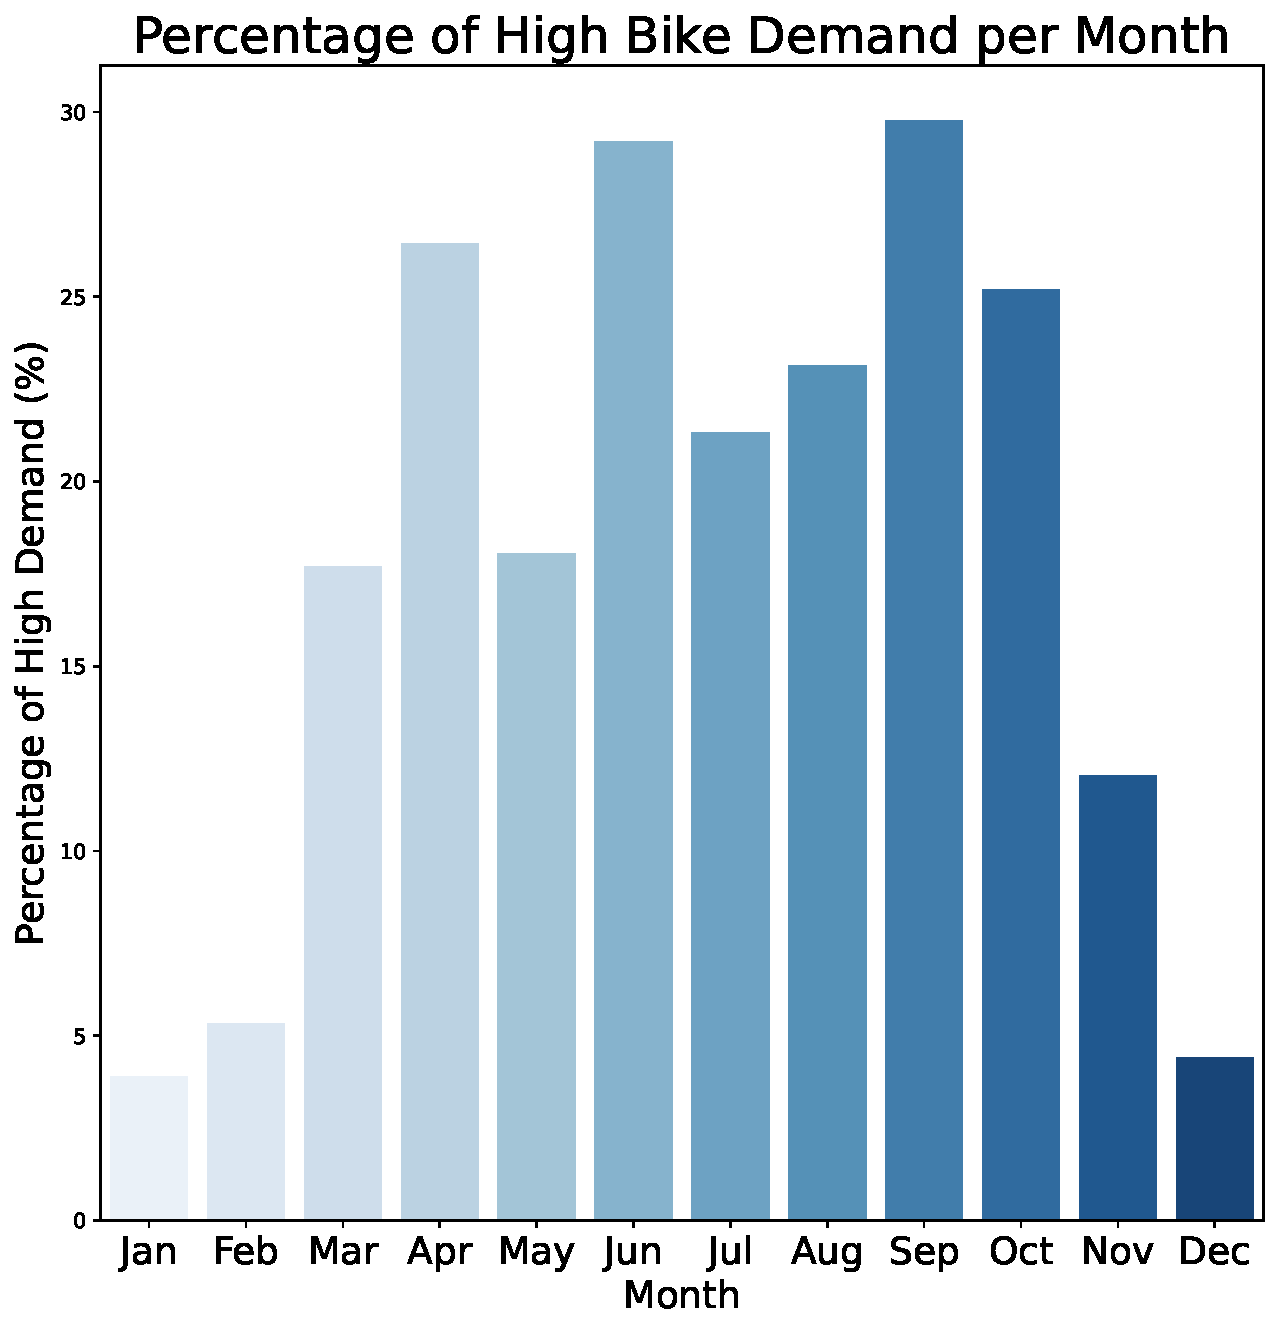
\includegraphics[width=\textwidth]{demand_month.pdf}
        \caption{Demand per month.}
        \label{fig:demand month}
    \end{subfigure}
    \hfill
    \begin{subfigure}{0.8\textwidth}
        \centering
        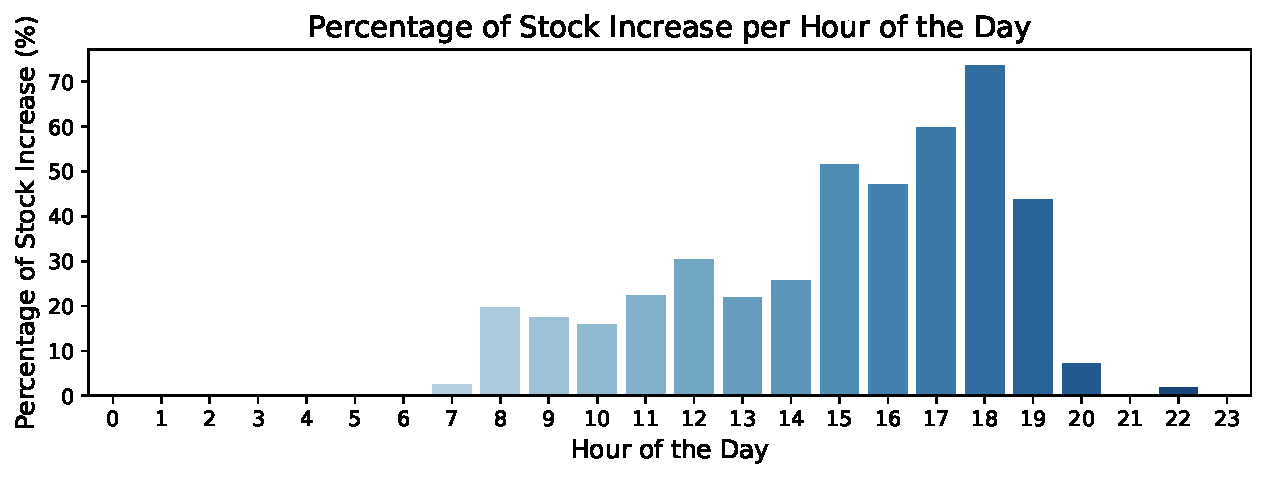
\includegraphics[width=\textwidth]{demand_hour.pdf}
        \caption{Demand per hour of day.}
        \label{fig:demand hour}
    \end{subfigure}
    \caption{Bike demand vs. day of week and month.}
    \label{fig:demand day month}
\end{figure}

\begin{figure}[htbp]
    \centering
    
    \caption{Bike demand vs. tempreature LÄGG IN FLER HÄR TYP.}
    \label{fig:demand time of day}
\end{figure}
% Gör en bra figure här med alla typ idk, även holiday.

There are some trends seen in the data when it comes to time and weather. From figure \ref{fig:demand day month}, one can see a periodic relationship for the months, where there is a higher demand during the warmer months, loosely following a trigonometric curve. Over the week, the demand is rather stable, with a peak on the weekend, especially saturdays. Looking at the weather; if there is rain or if there is snow on the ground, there is close to always low demand. Cloudcover did not make a big impact, which is also intuitive, as a cloudy day does not make biking more difficult. Dew point also does not have a clear trend, while humidity however has a clear trend downwards as the humidity increases.

The overall trend is that about one eigth of observations correspond to a high bike demand. During the night, or in bad weather, the demand is (intuitively) low. But during rush hour (fig. \ref{fig:demand time of day}), the demand is very high, and should probably be increased in order to minimize excessive CO$_2$ emissions.
%%%%%%%%%%%%%%%%%%%%%%%%%%%%%%%%%%%%%%
%%%%%%%%%%%%%%%%%%%%%%%%%%%%%%%%%%%%%%
%%%%%%%%%%%%%%%%%%%%%%%%%%%%%%%%%%%%%%
%%%%%%%%%%%%%%%%%%%%%%%%%%%%%%%%%%%%%%
%%%%%%%%%%%%%%%%%%%%%%%%%%%%%%%%%%%%%%
\section{Introduction}
Statistical machine learning is a subject that aims to build and train algorithms, that analyse large amount of data, and make predictions for the future, which are computed by using established statistical models, and tools from functional analysis. This is a project in supervised, statistical machine learning, where several models were created, and trained, in order to analyse which one of them gives best prediction for the project "Do we need more bikes", where we want to understand, and predict if there is a high, or low demand of city bikes in the public transportation of Washington, a project by the District Department of Transportation in Washington D.C..

The data set used for training our models, consist of 15 variables, containing quantitative/qualitative data. We developed several models, and evaluated them with cross-validation, in order to understand which algorithm gives the best prediction. 



%%%%%%%%%%%%%%%%%%%%%%%%%%%%%%%%%%%%%%
%%%%%%%%%%%%%%%%%%%%%%%%%%%%%%%%%%%%%%
%%%%%%%%%%%%%%%%%%%%%%%%%%%%%%%%%%%%%%
%%%%%%%%%%%%%%%%%%%%%%%%%%%%%%%%%%%%%%
%%%%%%%%%%%%%%%%%%%%%%%%%%%%%%%%%%%%%%
\section{Data analysis}

















%%%%%%%%%%%%%%%%%%%%%%%%%%%%%%%%%%%%%%
%%%%%%%%%%%%%%%%%%%%%%%%%%%%%%%%%%%%%%
%%%%%%%%%%%%%%%%%%%%%%%%%%%%%%%%%%%%%%
%%%%%%%%%%%%%%%%%%%%%%%%%%%%%%%%%%%%%%
%%%%%%%%%%%%%%%%%%%%%%%%%%%%%%%%%%%%%%
\section{Theoretical Background}


\subsection{Mathematical Overview of the Models}
    \subsubsection{Logistic Regression}
    The backbone of logistic regression is linear regression, i.e. finding the least-squares solution to an equation system \begin{equation}
        X\theta = y
    \end{equation}
    given by the normal equations \begin{equation}
        X^TX \theta = X^Ty
    \end{equation}
    where $X$ is the training data matrix, $\theta$ is the coefficient vector and $b$ is the training output. The parameter vector is then used in the sigmoid function: \begin{align}
        \sigma(z) &= \frac{e^{z}}{1+e^{z}}: \; \mathbb{R}\to [0,1],\\
        z &= x^T \theta,
    \end{align}
    where $x$ is the testing input. This gives a statistical interpretation of the input vector. In the case of a binary True/False classification, the value of the sigmoid function then determines the class.

\subsubsection{Random forest}

The random forest method is a based upon decision trees, i.e. dividing the data point into binary groups based on Gini-impurity, entropy or classification error, Gini being the most common. 
These divisions are then used to create a binary tree shown in figure \ref(Tree) and where thee leaf-nodes are used to classify the target variables bases on the input. 
As of itself the dicition tree tends to have unsatisfying results which leads to methodes like random forest that boost its accuracy.

    %%%%%%%%%%%%%%%%%%%%%%%%%%%%%%%%
    %%%%%%%%%%%%%%%%%%%%%%%%%%%%%%%%
    %%%%%%%%%%%%%%%%%%%%%%%%%%%%%%%%
    %%%%%%%%%%%%%%%%%%%%%%%%%%%%%%%%
    %%%%%%%%%%%%%%%%%%%%%%%%%%%%%%%%
    \subsubsection{Non-parametric method: k--Nearest Neighbour}
        \emph{$k$-- Nearest Neighbour}($k$--NN) is a distance based method that takes a $k$ amount of points from the training data set, called \emph{neighbours}, computes the distance between them, then assumes that the predicted value $\hat{y}(x_{*})$ follows the trend of the $k$-- nearest neighbours. Since $k$--NN uses the training data explicitly it is also called a \emph{nonparametric} method.

    The $k$--NN method can be divided into several subcategories, inter alias \emph{classification} $k$--NN method, \emph{regression}  $k$--NN method. In this project, we are using the classification method, since we are trying to predict in which of the two classes low, or high demand, the given, and predicted data points belong.

    The classification  $k$--NN algorithm evaluates $\hat{y}(x_{*})$ by computing the most frequently occurring class among the $k$ nearest neighbours. Here, we try to identify whether a data point belong to the high demand-class. Denote $c=$ high demand class. For simplicity, assume Euclidean ambiance. Then
        \begin{equation*}
            \hat{y}(x_*) = \arg \max_{c}  \sum_{n \in \mathbb{N}} \chi_{(y_i = c)} ,
        \end{equation*}
    where $y_i$ is the class of the nearest neighbour,  $\chi$ is the characteristic function 
        \begin{equation*}
            \chi_{(y_i = c)} = 
            \begin{cases}
                1 \qquad \text{if } y_n = c, \\
                0 \qquad \text{otherwise}.
                
            \end{cases}
        \end{equation*}
    It is very common to use a weighted sum to predict the next value, i.e.
        \begin{equation*}
            \hat{y}(x_*) =  arg \max_{c}  \sum_{n \in \mathbb{N}} \frac{\chi_{(y_n = c)}}{d(x, x_n)},
        \end{equation*}
    where $d$ is the standard Euclidean metric, computing the distance between an input $x$, and a neighbour $x_n$. 

    When using this model it is important to choose an optimal $k$--value. There are several tests for this, here we implement \emph{uniform weighting}, and \emph{distance weighting}. The first algorithm creates a $k$--NN model for each new $k \in [1, 500]$, and trains the model with uniform weights, i.e. the contribution of all neighbours is equal. Similarly, the latter trains a $k$--NN classifier for each $k \in [1, 500]$, with the difference that it uses distance based weighting, i.e. closer neighbours have greater influence. After testing different upper boundaries for $k$, the two models gave good results in the interval $[1,500]$, see Figure \ref{fig:kNN_comparison}. From the figures, we can see that the second test gives a better value for $k$, since the plot follows smoother trend, in comparison to the uniform weighting test, which makes it easier to identify an optimal $k$ value ($k = 120$). Moreover, the distance weighting algorithm is providing results for larger values of $k$, that is for $k \in [1, 400)$ before the curve converges, while the uniform weighting algorithm converges earlier, when $k = 290$. This means that for large $k$, both test algorithms make prediction based on the most common class in the data set, instead of making prediction based on the behaviour of the neighbours. Thus for sufficiently large $k$, for any given data point, the model will consider unnecessarily large amount of neighbours, and the prediction will be evaluated to belong to the most frequent class. Since the distance weighting has a larger range of $k$--value, it should be more trustworthy.
    
    \begin{figure}[htbp]
        \centering
        \begin{subfigure}{0.45\textwidth}
            \centering
            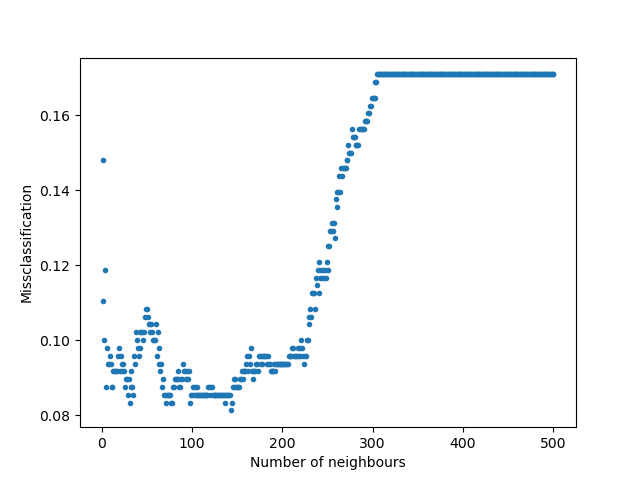
\includegraphics[width=\textwidth]{k-valueTest1ngh500.png}
            \caption{Uniform distance test for $k$.}
            \label{fig:kNN_fig1}
        \end{subfigure}
        \hfill
        \begin{subfigure}{0.45\textwidth}
            \centering
            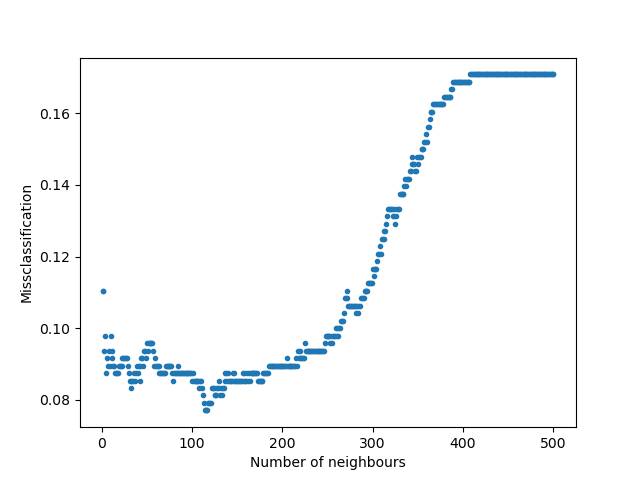
\includegraphics[width=\textwidth]{k-valueTest2ngh500.png}
            \caption{Weighted distance test for $k$.}
            \label{fig:kNN_fig2}
        \end{subfigure}
        \caption{Test for choosing an optimal $k$--value.}
        \label{fig:kNN_comparison}
    \end{figure}

    With the $k = 280$, the

    







    %%%%%%%%%%%%%%%%%%%%%%%%%%%%%%%%
    %%%%%%%%%%%%%%%%%%%%%%%%%%%%%%%%
    %%%%%%%%%%%%%%%%%%%%%%%%%%%%%%%%
    %%%%%%%%%%%%%%%%%%%%%%%%%%%%%%%%
    %%%%%%%%%%%%%%%%%%%%%%%%%%%%%%%%
    \subsection{Input Data Modification}
    \label{sec:input data modification}
    By plotting the data and analyzing the .csv file, some observations were made. The different inputs were then changed accordingly:
    \begin{itemize}
        \item \emph{Kept as-is}: \texttt{weekday}, \texttt{windspeed}, \texttt{visibility}, \texttt{temp}
        \item \emph{Modified}:
        \begin{itemize}
            \item \texttt{month} - split into two inputs, one cosine and one sine part. This make the new inputs linear and can follow the fluctuations of the year. The original input was discarded.
            \item \texttt{hour\_of\_day} - split into three boolean variables: \texttt{demand\_day}, \texttt{demand\_evening}, and \texttt{demand\_night}, reflecting if the time was between 08-14, 15-19 or 20-07 respectively. This was done because plotting the data showed three different plateaues of demand for the different time intervals. The original input was discarded.
            \item \texttt{snowdepth}, \texttt{precip} were transformed into booleans, reflecting if it was raining or if there was snow on the ground or not. This was done as there was no times where demand was high when it was raining or when there was snow on the ground.
        \end{itemize} 
        \item \emph{Removed}: \texttt{cloudcover}, \texttt{day\_of\_week}, \texttt{snow}, \texttt{dew}, \texttt{holiday}, \texttt{summertime}. These were removed due to being redundant (e.g. \texttt{summertime}), not showing a clear trend (e.g. \texttt{cloudcover}), giving a worse score when used, or all three (e.g. \texttt{day\_of\_week}).
    \end{itemize}
\section{Conclusion}

From the evaluation the two models k-nn performed the best with the highest accuracy and precision. 
As for the recall this is not the highest but is considered adequate and hence this method is chosen.
\\
\\
One reason for the discriminant analysis falling short of the other models is likely due to these models
being designed with the assumption of variables being normally distributed.
This is not the case for this particular data set.


\bibliography{ref.bib}
\appendix

  
\section*{Logistic regression method code}
\begin{lstlisting}[language = Python]

import numpy as np
import pandas as pd
import matplotlib.pyplot as plt
import sklearn.linear_model as skl_lm
import sklearn.preprocessing as pp
import sklearn.metrics as skl_m

df = pd.read_csv('training_data_vt2025.csv')
#df.info()

# Modify the dataset, emphasizing different variables
#df.iloc[:,12]=df.iloc[:,12]**2
#df.iloc[:,13]=np.sqrt(df.iloc[:,13])
#df.iloc[:,11] = df.iloc[:,11]**2

df['month_cos'] = np.cos(df.month*np.pi/12)
df['month_sin'] = np.sin(df.month*np.pi/12)

# time of day, replaed with low,medium and high demand, 
# adding the new categories back in the end.
def categorize_demand(hour):
    if 20 <= hour or 7 >= hour:
        return 'night'
    elif 8 <= hour <= 14:
        return 'day'
    elif 15 <= hour <= 19:
        return 'evening'

df['demand_category'] = df['hour_of_day'].apply(categorize_demand)
df_dummies = pd.get_dummies(df['demand_category'], prefix='demand', drop_first=False)
df = pd.concat([df, df_dummies], axis=1)

# converting to bools
def if_zero(data):
    if data == 0:
        return True
    else:
        return False

# temperature

df['snowdepth_bool'] = df['snowdepth'].replace(0, False).astype(bool)
df['precip_bool'] = df['precip'].replace(0, False).astype(bool)

# Split into train and test:

#df.iloc[:,15]=df.iloc[:,15].replace('low_bike_demand',False)
#df.iloc[:,15]=df.iloc[:,15].replace('high_bike_demand',True)
np.random.seed(0)

df_modified=df[[#'holiday',
                'weekday',
                #'summertime',
                'temp',
                #'dew',
                'humidity',
                'visibility',
                'windspeed',
                'month_cos',
                'month_sin',
                'demand_day',
                'demand_evening',
                'demand_night',
                'snowdepth_bool',
                'precip_bool',
                'increase_stock']]

N = df_modified.shape[0]
n = round(0.7*N)
trainI = np.random.choice(N,size=n,replace=False)
trainIndex = df_modified.index.isin(trainI)
train = df_modified.iloc[trainIndex]
test = df_modified.iloc[~trainIndex]

# Set up X,Y

# Train data 
X = train.iloc[:,0:-2]
Y = train['increase_stock']

# Test data
X_test = test.iloc[:,0:-2]
Y_test = test['increase_stock']

model = skl_lm.LogisticRegression()

# Scaling the data, otherwise
scaler = pp.StandardScaler().fit(X)
model.fit(scaler.transform(X),Y)
y_hat = model.predict(scaler.transform(X_test))

'''
# oskalad data
model.fit(X,Y)
y_hat = model.predict(X_test)'''

# Get confusion matrix
diff = pd.crosstab(y_hat, Y_test)
print(f'Confusion matrix: \n {diff}')

# No. of TP,TN,FP,FN
'''TP = diff.iloc[0,0]
TN = diff.iloc[1,1]
FP = diff.iloc[1,0]
FN = diff.iloc[0,1]'''

# Get metrics:
print(skl_m.classification_report(Y_test, y_hat))
   
\end{lstlisting}



\section*{Random forest code}
\begin{lstlisting}[language = Python]

    import pandas as pd
import numpy as np
import matplotlib
import matplotlib.pyplot as plt
from sklearn import tree
from sklearn.ensemble import BaggingClassifier, RandomForestClassifier
import graphviz
from sklearn.model_selection import GridSearchCV, RandomizedSearchCV
from sklearn.metrics import classification_report

df = pd.read_csv('training_data_vt2025.csv')
#df.info()

# Modify the dataset, emphasizing different variables
df.iloc[:,12]=df.iloc[:,12]**2
df.iloc[:,13]=np.sqrt(df.iloc[:,13])
df.iloc[:,11] = df.iloc[:,11]**2

df['month_cos'] = np.cos(df.month*np.pi/12)
df['month_sin'] = np.sin(df.month*np.pi/12)

# time of day, replaed with low,medium and high demand, 
# adding the new categories back in the end.
def categorize_demand(hour):
    if 20 <= hour or 7 >= hour:
        return 'night'
    elif 8 <= hour <= 14:
        return 'day'
    elif 15 <= hour <= 19:
        return 'evening'

df['demand_category'] = df['hour_of_day'].apply(categorize_demand)
df_dummies = pd.get_dummies(df['demand_category'], prefix='demand', drop_first=False)
df = pd.concat([df, df_dummies], axis=1)

# converting to bools
def if_zero(data):
    if data == 0:
        return True
    else:
        return False

# temperature

df['snowdepth_bool'] = df['snowdepth'].replace(0, False).astype(bool)
df['precip_bool'] = df['precip'].replace(0, False).astype(bool)

# Split into train and test:

#df.iloc[:,15]=df.iloc[:,15].replace('low_bike_demand',False)
#df.iloc[:,15]=df.iloc[:,15].replace('high_bike_demand',True)
np.random.seed(0)

df_modified=df[[#'holiday',
                'weekday',
                #'summertime',
                'temp',
                #'dew',
                #'humidity',
                'visibility',
                'windspeed',
                'month_cos',
                'month_sin',
                'demand_day',
                'demand_evening',
                'demand_night',
                'snowdepth_bool',
                'precip_bool',
                'increase_stock']]

N = df_modified.shape[0]
n = round(0.7*N)
trainI = np.random.choice(N,size=n,replace=False)
trainIndex = df_modified.index.isin(trainI)
train = df_modified.iloc[trainIndex]
test = df_modified.iloc[~trainIndex]

X_train = train.drop(columns=['increase_stock'])
# Need to transform the qualitative variables to dummy variables 

y_train = train['increase_stock']

model = RandomForestClassifier(random_state=42)
param_grid = {
    'n_estimators': [100, 200, 300], 
    'max_depth': [10, 20, None],     
    'min_samples_split': [2, 5, 10], 
    'min_samples_leaf': [1, 2, 4]     
}

# Set up Grid Search
random_search = RandomizedSearchCV(model, param_grid, cv=5, scoring='accuracy', n_jobs=-1, verbose=2)

# Fit on training data
random_search.fit(X_train, y_train)

# Get the best hyperparameters
print("Best Parameters: ", random_search.best_params_)
print("Best Accuracy: %.2f" % random_search.best_score_)

# Update the model with the best parameters
best_model = random_search.best_estimator_

# Fit the best model on the training data
best_model.fit(X_train, y_train)

# Make predictions using the optimized model




###
#dot_data = tree.export_graphviz(model, out_file=None, feature_names = X_train.columns,class_names = model.classes_, 
#                                filled=True, rounded=True,leaves_parallel=True, proportion=True)
#graph = graphviz.Source(dot_data)
#graph.render("decision_tree", format="pdf")
X_test = test.drop(columns=['increase_stock'])
y_test = test['increase_stock']
y_predict = best_model.predict(X_test)



print(classification_report(y_test, y_predict))
\end{lstlisting}



\section*{k-NN code}
\begin{lstlisting}[language = Python]

    import numpy as np
import pandas as pd
import matplotlib.pyplot as plt
import sklearn.linear_model as skl_lm
import sklearn.preprocessing as pp
import sklearn.metrics as skl_m

import sklearn.neighbors as skl_nb

df = pd.read_csv('training_data_vt2025.csv')
#df.info()

# Modify the dataset, emphasizing different variables
#df.iloc[:,12]=df.iloc[:,12]**2
#df.iloc[:,13]=np.sqrt(df.iloc[:,13])
#df.iloc[:,11] = df.iloc[:,11]**2

df['month_cos'] = np.cos(df.month*np.pi/12)
df['month_sin'] = np.sin(df.month*np.pi/12)

# time of day, replaed with low,medium and high demand, 
# adding the new categories back in the end.
def categorize_demand(hour):
    if 20 <= hour or 7 >= hour:
        return 'night'
    elif 8 <= hour <= 14:
        return 'day'
    elif 15 <= hour <= 19:
        return 'evening'

df['demand_category'] = df['hour_of_day'].apply(categorize_demand)
df_dummies = pd.get_dummies(df['demand_category'], prefix='demand', drop_first=False)
df = pd.concat([df, df_dummies], axis=1)

# converting to bools
def if_zero(data):
    if data == 0:
        return True
    else:
        return False

# temperature

df['snowdepth_bool'] = df['snowdepth'].replace(0, False).astype(bool)
df['precip_bool'] = df['precip'].replace(0, False).astype(bool)

# Split into train and test:

#df.iloc[:,15]=df.iloc[:,15].replace('low_bike_demand',False)
#df.iloc[:,15]=df.iloc[:,15].replace('high_bike_demand',True)
np.random.seed(0)

df_modified=df[[#'holiday',
                'weekday',
                #'summertime',
                'temp',
                #'dew',
                'humidity',
                'visibility',
                'windspeed',
                'month_cos',
                'month_sin',
                'demand_day',
                'demand_evening',
                'demand_night',
                'snowdepth_bool',
                'precip_bool',
                'increase_stock']]

N = df_modified.shape[0]
n = round(0.7*N)
trainI = np.random.choice(N,size=n,replace=False)
trainIndex = df_modified.index.isin(trainI)
train = df_modified.iloc[trainIndex]
test = df_modified.iloc[~trainIndex]

# Set up X,Y

# Train data 
X = train.iloc[:,0:-2]
Y = train['increase_stock']

# Test data
X_test = test.iloc[:,0:-2]
Y_test = test['increase_stock']


"""
# Tests for k-value
# TEST 1 - uniform distance
missclassification = []
for k in range(500): # Try n_neighbours = 1, 2, ....,

    #kNN method
    scaler = pp.StandardScaler().fit(X)
    model = skl_nb.KNeighborsClassifier(n_neighbors = k+1, weights = 'uniform')
    model.fit(scaler.transform(X),Y)

    # Prediction
    y_hat = model.predict(scaler.transform(X_test))
    missclassification.append(np.mean(y_hat != Y_test))

K = np.linspace(1, 500, 500)
plt.plot(K, missclassification, '.')
plt.ylabel('Missclassification')
plt.xlabel('Number of neighbours')
plt.show()

#TEST 2
missclassification = []
for k in range(500): # Try n_neighbours = 1, 2, ....,

    #kNN method
    scaler = pp.StandardScaler().fit(X)
    model = skl_nb.KNeighborsClassifier(n_neighbors = k+1, weights = 'distance')
    model.fit(scaler.transform(X),Y)

    # Prediction
    y_hat = model.predict(scaler.transform(X_test))
    missclassification.append(np.mean(y_hat != Y_test))

K = np.linspace(1, 500, 500)
plt.plot(K, missclassification, '.')
plt.ylabel('Missclassification')
plt.xlabel('Number of neighbours')
plt.show()
"""



# creating the model
model = skl_nb.KNeighborsClassifier(n_neighbors = 120, weights = 'distance')


# Scaling the data, otherwise
scaler = pp.StandardScaler().fit(X)
model.fit(scaler.transform(X),Y)
y_hat = model.predict(scaler.transform(X_test))



'''
# oskalad data
model.fit(X,Y)
y_hat = model.predict(X_test)'''

# Get confusion matrix
diff = pd.crosstab(y_hat, Y_test)
print(f'Confusion matrix: \n {diff}')

# No. of TP,TN,FP,FN
'''TP = diff.iloc[0,0]
TN = diff.iloc[1,1]
FP = diff.iloc[1,0]
FN = diff.iloc[0,1]'''

# Get metrics:
print(skl_m.classification_report(Y_test, y_hat))
\end{lstlisting}




\section*{QDA code}
\begin{lstlisting}[language = Python]

    import pandas as pd
import numpy as np
from sklearn.model_selection import train_test_split
from sklearn.discriminant_analysis import QuadraticDiscriminantAnalysis
from sklearn.metrics import accuracy_score
from sklearn.metrics import classification_report

df = pd.read_csv('training_data_vt2025.csv')

# modify the month to represent the periodicity that is observed in data.
df['month_cos'] = np.cos(df['month']*2*np.pi/12)
df['month_sin'] = np.sin(df['month']*2*np.pi/12)

# time of day, replaced with 3 bool values: is_night, is_day and is_evening, 
# adding the new categories back in the end.
def categorize_demand(hour):
    if 20 <= hour or 7 >= hour:
        return 'night'
    elif 8 <= hour <= 14:
        return 'day'
    elif 15 <= hour <= 19:
        return 'evening'

df['time_of_day'] = df['hour_of_day'].apply(categorize_demand)
df_dummies = pd.get_dummies(df['time_of_day'], prefix='is', drop_first=False)
df = pd.concat([df, df_dummies], axis=1)

# Create bool of snowdepth and percipitation
df['snowdepth_bool'] = df['snowdepth'].where(df['snowdepth'] == 0, 1)
df['precip_bool'] = df['precip'].where(df['precip'] == 0, 1)

# Seperate training data from target
X=df[[#'holiday',
        'weekday',
        #'summertime',
        'temp',
        #'dew',
        #'humidity',
        #'visibility',
        #'windspeed',
        #'month',
        'month_cos',
        'month_sin',
        #'hour_of_day',
        'is_day',
        'is_evening',
        'is_night',
        #'snowdepth_bool',
        'precip_bool'
        ]]

y=df['increase_stock']

# Split dataset into training and test sets
X_train, X_test, y_train, y_test = train_test_split(X, y, test_size=0.2, random_state=42)

# Apply Quadratic Discriminant Analysis (QDA)
qda = QuadraticDiscriminantAnalysis() 
X_train_lda = qda.fit(X_train, y_train)

# Make predictions
y_pred = qda.predict(X_test)

# Evaluate accuracy
accuracy = accuracy_score(y_test, y_pred)
print(f"Model Accuracy: {accuracy:.2f}")

print(classification_report(y_test, y_pred))
\end{lstlisting}



%\lstinputlisting[language=python]{code.py} % lägg in i appendix typ?



\end{document}